\documentclass[12pt]{article}
\usepackage[top=1in, bottom=1in, right=1in, left=1in]{geometry}
\usepackage{setspace}
\usepackage{graphicx}
\usepackage{setspace}
\usepackage{parskip}
\usepackage{url}

\title{Excepted Appointments and Presidential Unilateral Power}
\date{February 2, 2016}
\author{Emily H. Moore}


\usepackage{Sweave}
\begin{document}
\Sconcordance{concordance:ExceptedAppointmentsandPresidentialUnilateralPowersFeb12016.tex:ExceptedAppointmentsandPresidentialUnilateralPowersFeb12016.Rnw:%
1 13 1 1 0 266 1}

\maketitle
\parindent=0.5in
\parskip=0.01in
\doublespacing

%%Things I still need to do on this:


Presidents use a variety of tools to influence both legislative and administrative policymaking. They can experience greater legislative success in Congress by exercising their veto powers (Cameron 2000) and leveraging bureaucratic expertise (Howell, Jackman, and Rogowski 2013). Presidents may create policy without Congress using executive orders, proclamations, national security directives, and executive agreements (e.g., Howell 2003). They  also possess an extensive array of tools for managing the bureaucracy, which can enable them to exploit informational advantages (Gailmard and Patty 2012), regulate strategically (e.g., O'Connell 2008; Yackee and Yackee 2009a, 2009b), and appoint personnel of their choosing (e.g., Lewis 2008). 

	As Moe (1985) argues, presidents have incentives to use their appointment power to politicize the bureaucracy. They do this because administrative control creates power for presidents to pursue their agendas and allows them to bargain more effectively with other institutions.  Lewis (2008, 2011) shows that presidents bolster this administrative control by increasing the number of appointments available to them, expanding appointment power in key management positions, and strategically placing appointments in agencies with unfavorable politics. Virtually everything we know about the appointment power, however, is based on studies of the very small portion of appointees who undergo Senate confirmation. This is surprising given that the vast majority of bureaucrats are not subject to Senate confirmation but nonetheless perform important functions within the bureaucracy.
	
	To illustrate the importance of excepted appointees, consider the case of Antonio Weiss and the Department of the Treasury. In November 2014, President Obama nominated Weiss, head of investment banking for independent financial management firm Lazard, as the Undersecretary for Domestic Finance. Led by Elizabeth Warren, a number of progressive Democrats in the Senate opposed Weiss' appointment.\footnote{ These Democrats were concerned about Weiss' financial industry ties, believing he may not be willing to produce stringent enough regulations. More information can be found in this article: http://www.politico.com/story/2015/01/antonio-weiss-pulls-out-treasury-undersecretary-114191\\} To avoid a confirmation showdown, Obama withdrew the nomination and instead appointed Weiss as Counselor to the Secretary of the Treasury, a position which does not require Senate confirmation. While he may have fewer formal responsibilities as Counselor than he would have as Undersecretary, Weiss had the ability to affect policy immediately rather than risking a lengthy and potentially unsuccessful confirmation battle.	\footnote{ Elizabeth Warren should especially appreciate the importance of these lower-level positions because she served as an excepted Schedule C appointee under Secretary Geithner, appointed for the express purpose of creating the Consumer Financial Protection Bureau. Lewis (2011) argues that Warren was appointed as a Schedule C to specifically avoid a contentious fight in the Senate.}
	
	This episode illustrates two aspects of excepted appointees that make them powerful weapons in the president's unilateral policy arsenal. The first is flexibility. Rather than wait months for appointments to be confirmed and risk potential embarrassment if they are not, presidents can appoint officials who will pursue their agendas immediately.  In addition to the difficulties caused by confirmation delays, there may be instances in which positions must be filled quickly in order to fulfill essential tasks in an agency. New agencies related to the president's agenda need the capacity to act, sometimes without waiting for the confirmation process to occur. The second important aspect relates to politicization. As the Warren-Weiss example shows, presidents can use excepted appointments to appoint individuals that Congress could not or would not confirm. In one instance, Congress may oppose an appointee, leading the president to find other means to hire his preferred candidate. In another, gridlock may prevent Congress from confirming a nominee desirable to a majority of members.
	
	In this paper, I argue that excepted appointees\footnote{As I mention in greater detail in later sections, excepted service appointments are technically those individuals who are not appointed through the competitive hiring process. However, in practice, OPM does not refer to all such employees as excepted. Senate-confirmed appointees carry the distinction``PAS." Most of the excepted service positions to which OPM refers are excepted both from the competitive processes and advice and consent, which is how I choose to use the term.} are consequential tools in the president's unilateral policy arsenal. While excepted appointments lack the glamour and intrigue associated with their PAS counterparts, they are nonetheless responsible for carrying out vital agency tasks. In fact, because these Schedule C appointees are ``invisible" (Lewis and Waterman 2013), they largely fly under the radar of congressional and media oversight, allowing the president to use them with relatively few restrictions. This makes excepted appointments an important component of presidential unilateral power--an aspect which studies on unilateralism have largely overlooked in favor of more visible assertions of this power, like executive orders, memoranda, or warmaking. Indeed, because the president cares about exerting his influence over the executive branch as a whole, scholars must focus on the many variations this power can take and excepted appointments are one such form. 

		To remedy this gap in the literature, I introduce a dataset of all Schedule C appointments from 1998 to 2013. Examining changes in the number of Schedule C appointments, I show preliminary evidence that presidents may use these appointments to quickly fill positions for which Senate confirmation would take much longer. I also show that presidents utilize Schedule C appointments to advance their agendas, increasing the number of Schedule C appointees in ideologically similar agencies. In combination, these results show that Schedule C appointees offer the president the flexibility he needs to fill positions quickly with ideological allies.
		
\section*{The Politics of Staffing the Bureaucracy}

%%More specificity here?
	As a long history of literature on bureaucratic management and staffing suggests, presidents care about how agencies execute policy. Much scholarly work is devoted to the president's tradeoff between competent ``experts" and political loyalists (e.g. Heclo 1977; Hollibaugh et al. 2014; Lewis 2008; Moe 1985; Parsneau 2013). While the former may attempt to shift policy closer to their own view points and away from the president's (Moe 1985), the latter may lack the skill to execute policy well or efficiently (e.g. Lewis 2005; Gilmour and Lewis 2006; Heclo 1975, 1977). Apart from ideology and competence, the president also considers patronage when making hiring decisions (Lewis 2008; Hollibaugh et al. 2014). Because different appointment types have different uses for the president, he must decide how and where to best utilize them. One body of literature explores this decisionmaking process (e.g. Hollibaugh et al. 2014; Lewis and Waterman 2013; Patterson 2008; Patterson and Pfiffner 2001; Tolchin and Tolchin 2010). For example, Hollibaugh et al. (2014) find that presidents place patronage appointees in agencies on the president's agenda but where they have little ability to affect policy. Scholars have been particularly concerned with a tendency for the president to ``politicize" the bureaucracy--that is, use appointees selected based on their ties to the party rather than expertise. (e.g., Burke 1992; Hart 1995; Heclo 1975; Lewis 2005, 2008; Wayne et al. 1979). While competence still plays a role, ideology is undeniably a part of the president's attempts to gain administrative control. Because they worry that appointees selected on competence will not support them ideologically, presidents are continually trying to use their appointees to control more than just the leadership of the bureaucracy (Lewis 2008).

Lewis (2008) provides important insights into how presidents politicize. He finds that many appointment types are concentrated in ideologically opposed agencies, but Schedule C appointees may be concentrated both in ideologically close and distant agencies. He argues at times presidents may wish to use the more flexibile nature of Schedule C appointees to fill important positions in ideologically dissimilar agencies, but at other times, they may place Schedule C appointees in similar agencies for patronage purposes. However, the presence of Schedule C appointees in ideologically similar agencies is not dispositive of patronage. Indeed, the president needs appointees at all levels to help carry out the policies on his agenda and these policies may well be carried through by agencies ideologically aligned with the president. Moreover, as Lewis (2008) admits, appointees appointed for patronage reasons may also be appointed for other reasons, such as their ideological alignment with the president, and having a patronage component to an appointment does not mean that appointee is unable to affect policy. 

Presidents use higher-level appointees to help carry out policies on their agenda, but they also utilize excepted appointees. Lower level appointees are often responsible for making important policy decisions or carrying out vital agency tasks. Without these lower level appointees, it may be impossible to enact the president's agenda. In an interview, President Ford argued for greater appointment power at the lower levels of the bureaucracy, stating, ``if he [the president] cannot reach into the bowels of a department his decisions way up at the top will seldom be adequately implemented out in the grass roots" (Lewis 2008, 57). Despite their usefulness to the president, lower-level appointees, and especially those who do not face Senate confirmation, generally have been overlooked in bureaucracy scholarship.

The president's ability to appoint Schedule Cs is also an illustration of the first-mover advantage. Howell (2003) claims that one of the major advantages of presidential unilateral action is not merely for the president to act alone but also in his ability to act first, forcing Congress to react to his own actions. Schedule Cs may also provide this advantage. For example, presidents may fill new agencies with their own appointees, allowing them to set policy before Congress finishes approving more traditional appointment types. Agencies may also be faced with exogenous circumstances on which Congress and the president want them to act. If the president has the opportunity to place and direct his own appointees before Congress has a chance to respond, the president's appointees may set policies in motion Congress has difficulty changing.
	
While the president considers ideological alignment of appointees and agencies when he makes hiring decisions, it is easy to imagine other factors that influence staffing as well. For example, an agency's size or mission may necessitate a larger number of political appointees. A large and geographically dispersed employee base may require a greater number of political managers. Another non-ideological consideration is flexibility. Presidents come to office with agendas, but outside events may quickly alter their priorities. Appointments are one way to help guide agencies when unexpected challenges arrive. Examining both ideology and flexibility as important parts of staffing decisions will help us learn more about bureaucratic management, especially to the extent that these decisions occur outside congressional purview. 
	
\subsubsection*{Flexibility}

Given the difficulties of the advice and consent process, it is easy to imagine why presidents need flexibility. As alluded to before, delay and failure are the two most obvious of many confirmation troubles. In a recent study, Anne Joseph O'Connell (2015) finds that the length of time to confirmation has increased substantially since the 1980s. Obama's nominees waited twice as long to be confirmed as Reagan's. Moreover, over 25 percent of presidential nominations failed since the 1980s with greater failure rates for Bush and Obama than their predecessors. She also found that the nuclear option implemented in 2013 decreased wait times for judicial nominees, but increased wait times for all other agencies at the same time. This is especially important given the increasing length of time to confirmation and falling success rates for PAS appointees. The average JFK appointee waited only 2.5 months to be confirmed by the Senate while the average George W. Bush appointee waited nine months. Reagan appointed 86 percent of his top officials in his first year, but Obama could not complete two-thirds (Pfiffner 2015). Lengthy confirmation ordeals could severely hinder the president's agenda (Lewis 2011; McCarty and Razaghian 1999). One \textit{Washington Post} article (Eilperin 2014) describes just how damaging wait times can be late in a presidency. While confirmation rates are similar to other presidents, Obama's nominees have waited an average of 265 days to be confirmed, leaving little time, Eilperin argues, for nominees to be successfully confirmed and then little time to actually work in the administration. Describing the confirmation process as ``a living purgatory," the chief executive of the Partnership for Public Service explained that the process has dissuaded some of the very best candidates from applying. If candidates are not from the DC area already, the cost of the confirmation process for nominees is considerable. One law professor from Indiana rented a home in Maryland and commuted back and forth at her own expense, waiting 14 months for a confirmation vote which never occurred. She finally had her nomination withdrawn. Because of these considerable expenses, long waits dissuade all but those in the DC area or who are wealthy enough to survive. This limits the president's options and deters talented people from working in the administration (Eilperin 2014). Alternatively, the excepted service allows the president to select talented individuals who are unwilling or unable to undergo advice and consent. 

An increase in the length of time to confirmation also means an increase in the time to filling vacancies, which happens often given the relatively short amount of time appointees stay in their positions (O'Connell 2008; Pfiffner 2015). O'Connell (2008) finds that top positions in cabinet and executive agencies are vacant or filled by an acting official 15 to 25 percent of the time in recent years. O'Connell (2010) points out that missing leadership in agencies can lead to delays in the president's regulatory agenda, but she further argues that these vacancies leave room for excepted appointees to exercise greater influence over policy than they normally would.

%%PRESIDENT HINDERED BY LACK OF PERSONNEL?

While the president would clearly prefer Congress to quickly and easily confirm every appointee he desires, this is not always possible. At times, Congress may oppose the president's nominees for political reasons. One nominee for the EPA had waited more than 1,000 days because Republicans did not support one of the EPA's proposed rules and used his nomination as leverage to revoke it (Eilperin 2014). Moreover, confirmation battles are not merely a problem for the president in times of divided government. While failure rates are worse, delay is typically the same whether or not the Senate majority shares the president's partisanship (O'Connell 2008). The president does not want his agenda to be held up by a lack of personnel. For this reason he may find it useful to use lower level appointees to fill in the gaps. Excepted appointments give him just this ability. As such, I hypothesize that the president will utilize Schedule C appointments when he needs personnel more urgently. For example, the president may fill positions in new and salient departments with Schedule C appointments while waiting for Congress to move on the higher up positions.

\subsection*{Ideology}

Some evidence suggests agencies vary in their policy views and willingness to follow the president's directives (Aberbach and Rockman 1976, 1995, 2000; Bertelli and Grose 2009; Clinton and Lewis 2008; Clinton et al. 2012; Hollibaugh et al. 2014). Given these considerations, it is difficult to reason whether presidents care more about staffing ideologically similar or dissimilar agencies. On the one hand, the president may wish to offset his ideological enemies by pouring appointeees into ideologically distant agencies. On the other hand, similar agencies are likely close to the president's party and agenda and need the capacity to act that staff may provide.

Evidence suggests that presidents take variations in bureau ideology into account when making hiring decisions. Knowing that Schedule C appointees are important to the president because of the information they are able to provide (Gailmard and Patty 2012), it is reasonable to believe the president would want Schedule C appointees in important positions within agencies pursuing his agenda. In other words, because ideologically similar agencies are often important to the president and his party, it makes sense that the president would want to bolster his ideological allies. Excepted appointees allow the president a unique opportunity to move agencies independent of congressional desires and sometimes in spite of them. I hypothesize that the president will consider both agency and appointee ideology in his hiring decisions, placing excepted appointees into more ideologically similar agencies.

\subsection*{Excepted Service and the Larger Appointment System}

	To better study excepted appointments, it is useful to understand how they fit in the appointment system. While most scholarship tends to focus on traditional advice and consent appointments, most jobs in the bureaucracy are filled through a competitive process open to the public just as industry jobs are filled. Excepted service positions are technically those appointments that have been excepted from the competitive hiring process. Positions like Schedule C or SES are also exempt from advice and consent.\footnote{Some excepted service appointments are reserved for positions for which the Office of Personnel Management (OPM) does not or cannot provide a test or standard (professionals such as lawyers are one example). Other excepted service appointments are reserved for those with disabilities or are set aside for interns. These appointments, like competitive service appointments, are largely used to complete the day-to-day operations of the government.}	Unlike many other excepted positions, Schedule C appointments are positions excepted for political reasons. OPM describes Schedule C appointments as those positions of a ``confidential" or ``policy-determining nature," for which it is important the employee shares the president's vision for the agency. Figure 1 puts agency hierarchy into perspective for the Department of Agriculture, showing one page of the Plum Book (U.S. House of Representatives 2012, 11).\footnote{The Plum Book is a government publication released once every four years by Congress. It began in the Eisenhower administration for the same reasons that he created Schedule C: because he did not have enough information about the bureaucracy. The Plum Book lists appointments available for the president to make. He can later add Schedule C positions not listed in the Plum Book.} PAS appointees occupy top positions. NA appointees (Non-career appointees, like SES) occupy many high positions, but Schedule Cs follow quickly.\footnote{The TA appointment is a temporary appointment.}
	
PAS appointees fill the seniormost positions in the Department of Agriculture. The Secretary of Agriculture, of course, is responsible for communicating with the president and dictating policy within the department. The Deputy Secretary works directly with the secretary to fulfill the policy goals for the agency and communicate them with the various sub-departments. The Department of Agriculture covers a vast array of policy areas--domestic and international trade and agriculture, food safety, nutrition, rural development, and more. Because of this policy breadth the Department has many Deputy Undersecretaries serving in these various sub-departments. These individuals are typically non-career SES appointees--senior officials who are also excepted from both advice and consent and the competitive civil service. These deputy undersecretaries are tasked with advising the more senior PAS staff on their individual policy areas. Schedule C appointees provide a wide array of services within agencies. Some serve as scheduling assistants and speech writers others serve as more important policy advisors. Special Assistants, for example, typically advise the deputy undersecretary on specific policy areas, but they may be asked to fill whatever current needs in the department may be. Schedule C chiefs of staff within sub-departments fill somewhat more important roles. They may brief deputy undersecretaries, control their schedules, fill in for them in their absence, approve rules created by career staff, and resolve disputes between employees. 
	
\begin{figure}[htb]
\begin{center}
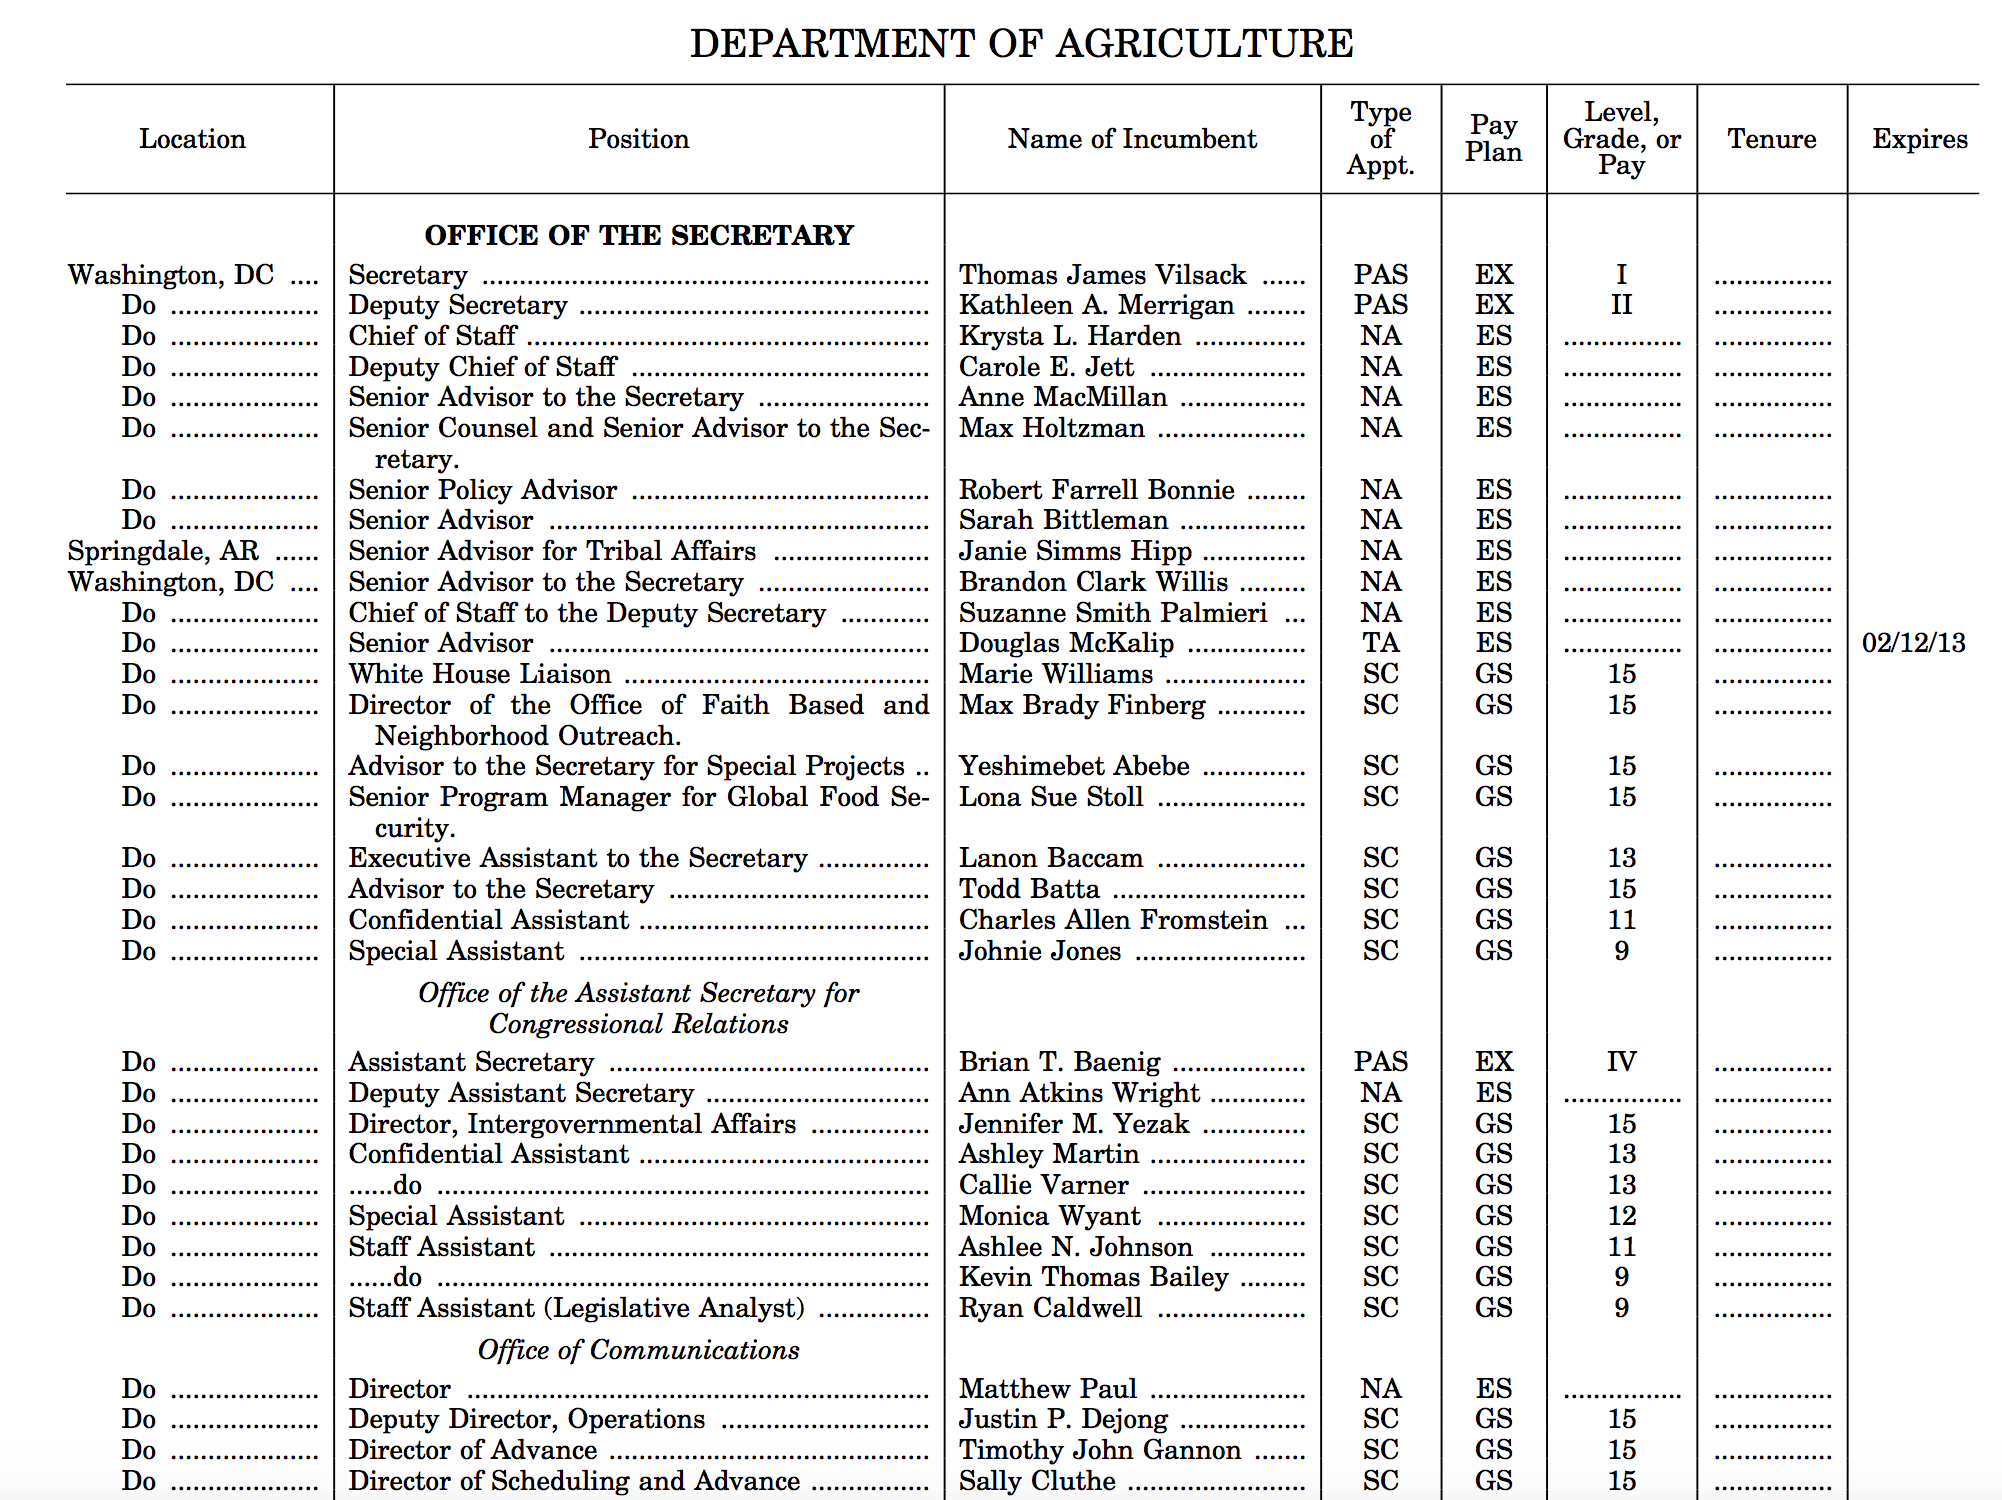
\includegraphics[height=5.5in,width=7in]{PlumBookPage.png}
\caption{Page from the Plum Book on the Department of Agriculture}
\end{center}
\end{figure}

	President Eisenhower created Schedule C appointments when he first reached office. According to Gailmard and Patty (2012), Eisenhower instituted Schedule C because he was faced with the political realities of being the first Republican to win the presidency in twenty years (leaving him with few trusted advisors) and because the post-World War II era left him with an expansive administrative state, which reached further into the economy and society than had previously been conceived. Schedule C was designed to exist between other classes of appointments---appointees beholden directly to the president, but who did not undergo advice and consent or competitive service processes. Today, Schedule C appointees make up about 15 percent of the president's available appointments in the Plum Book.
	
	Schedule C positions are created uniquely for each employee. When the administration wishes to hire someone via Schedule C, it files papers with OPM detailing the responsibilities of the position to justify a particular pay grade and describes its role within the home agency. When the Schedule C is fired or quits, the position is dissolved. If the administration wishes to hire another person to fulfill the role, it must file the paperwork to create the position anew. In other words, Schedule C appointees are not filling a statutory position; they are filling the administration's current needs.	
	
	Though Schedule C positions are not as prestigious as Senate-confirmed appointments, they can still have an impact on policy. Lewis and Waterman (2013) describe a Department of Justice investigation, which found that a Senior Executive Service and former Schedule C appointee, Monica Goodling, was involved in hiring, firing, and promoting civil servants on the basis of political views. Similar lower level appointees engaged in ``bullying career staff, censoring government reports, and leaking internal documents to outside groups in order to pursue the administration's policy and political goals" (Lewis and Waterman 2013, pg. 36). Lewis and Waterman go on to note of Goodling that despite her ``low" status, she ``initiated a series of crucial, politically and legally questionable decisions" (pg. 36). 
	
\section*{Excepted Service 1998-2013}

The federal employment and accessions data come from the FedScope tool through the Office of Personnel Management.\footnote{OPM refers to Fedscope as the Enterprise Human Resources Integration-Statistical Data Mart (EHRI-SDM).} From the FedScope tool, I collected static data on employment statistics for September 1998-2013. These data are a picture-in-time of employment in federal agencies, representing the total employment to each included agency for September of the given year. Over the period, there were 692 agency units, some of which were created or disbanded during the time period. These are counted based on which agencies have unique agency codes (given by OPM) in the data. \footnote{Most cabinet agencies provide data below the department level. For example, the Department of Defense is massive and includes sub-departments for the Army, Navy, Air Force, and general DOD and within these departments there are unique agencies bearing the department prefix. For example, the Air Force bears the prefix "AF" so the Air Force Operational Test and Evaluation Center is labeled "AF03." The State Department and Department of Energy do not provide data at the sublevel. Most independent agencies (e.g. EPA or SEC) do not provide data below the overall agency level, although a few do. The FedScope database is fairly comprehensive. However, it does exclude intelligence agencies and the U.S. Postal Service in its reporting, so it is not a complete representation of every federal employee. The State Department also does not report on Foreign Service Personnel.}

Figure 2 displays the number of Schedule C appointees from 1998-2013 and the number of Schedule C accessions (new hires and transfers) from 2005-2013. Unfortuantely, FedScope does not report accessions data prior to FY2005. 

\begin{figure}[!htb]
\begin{center}
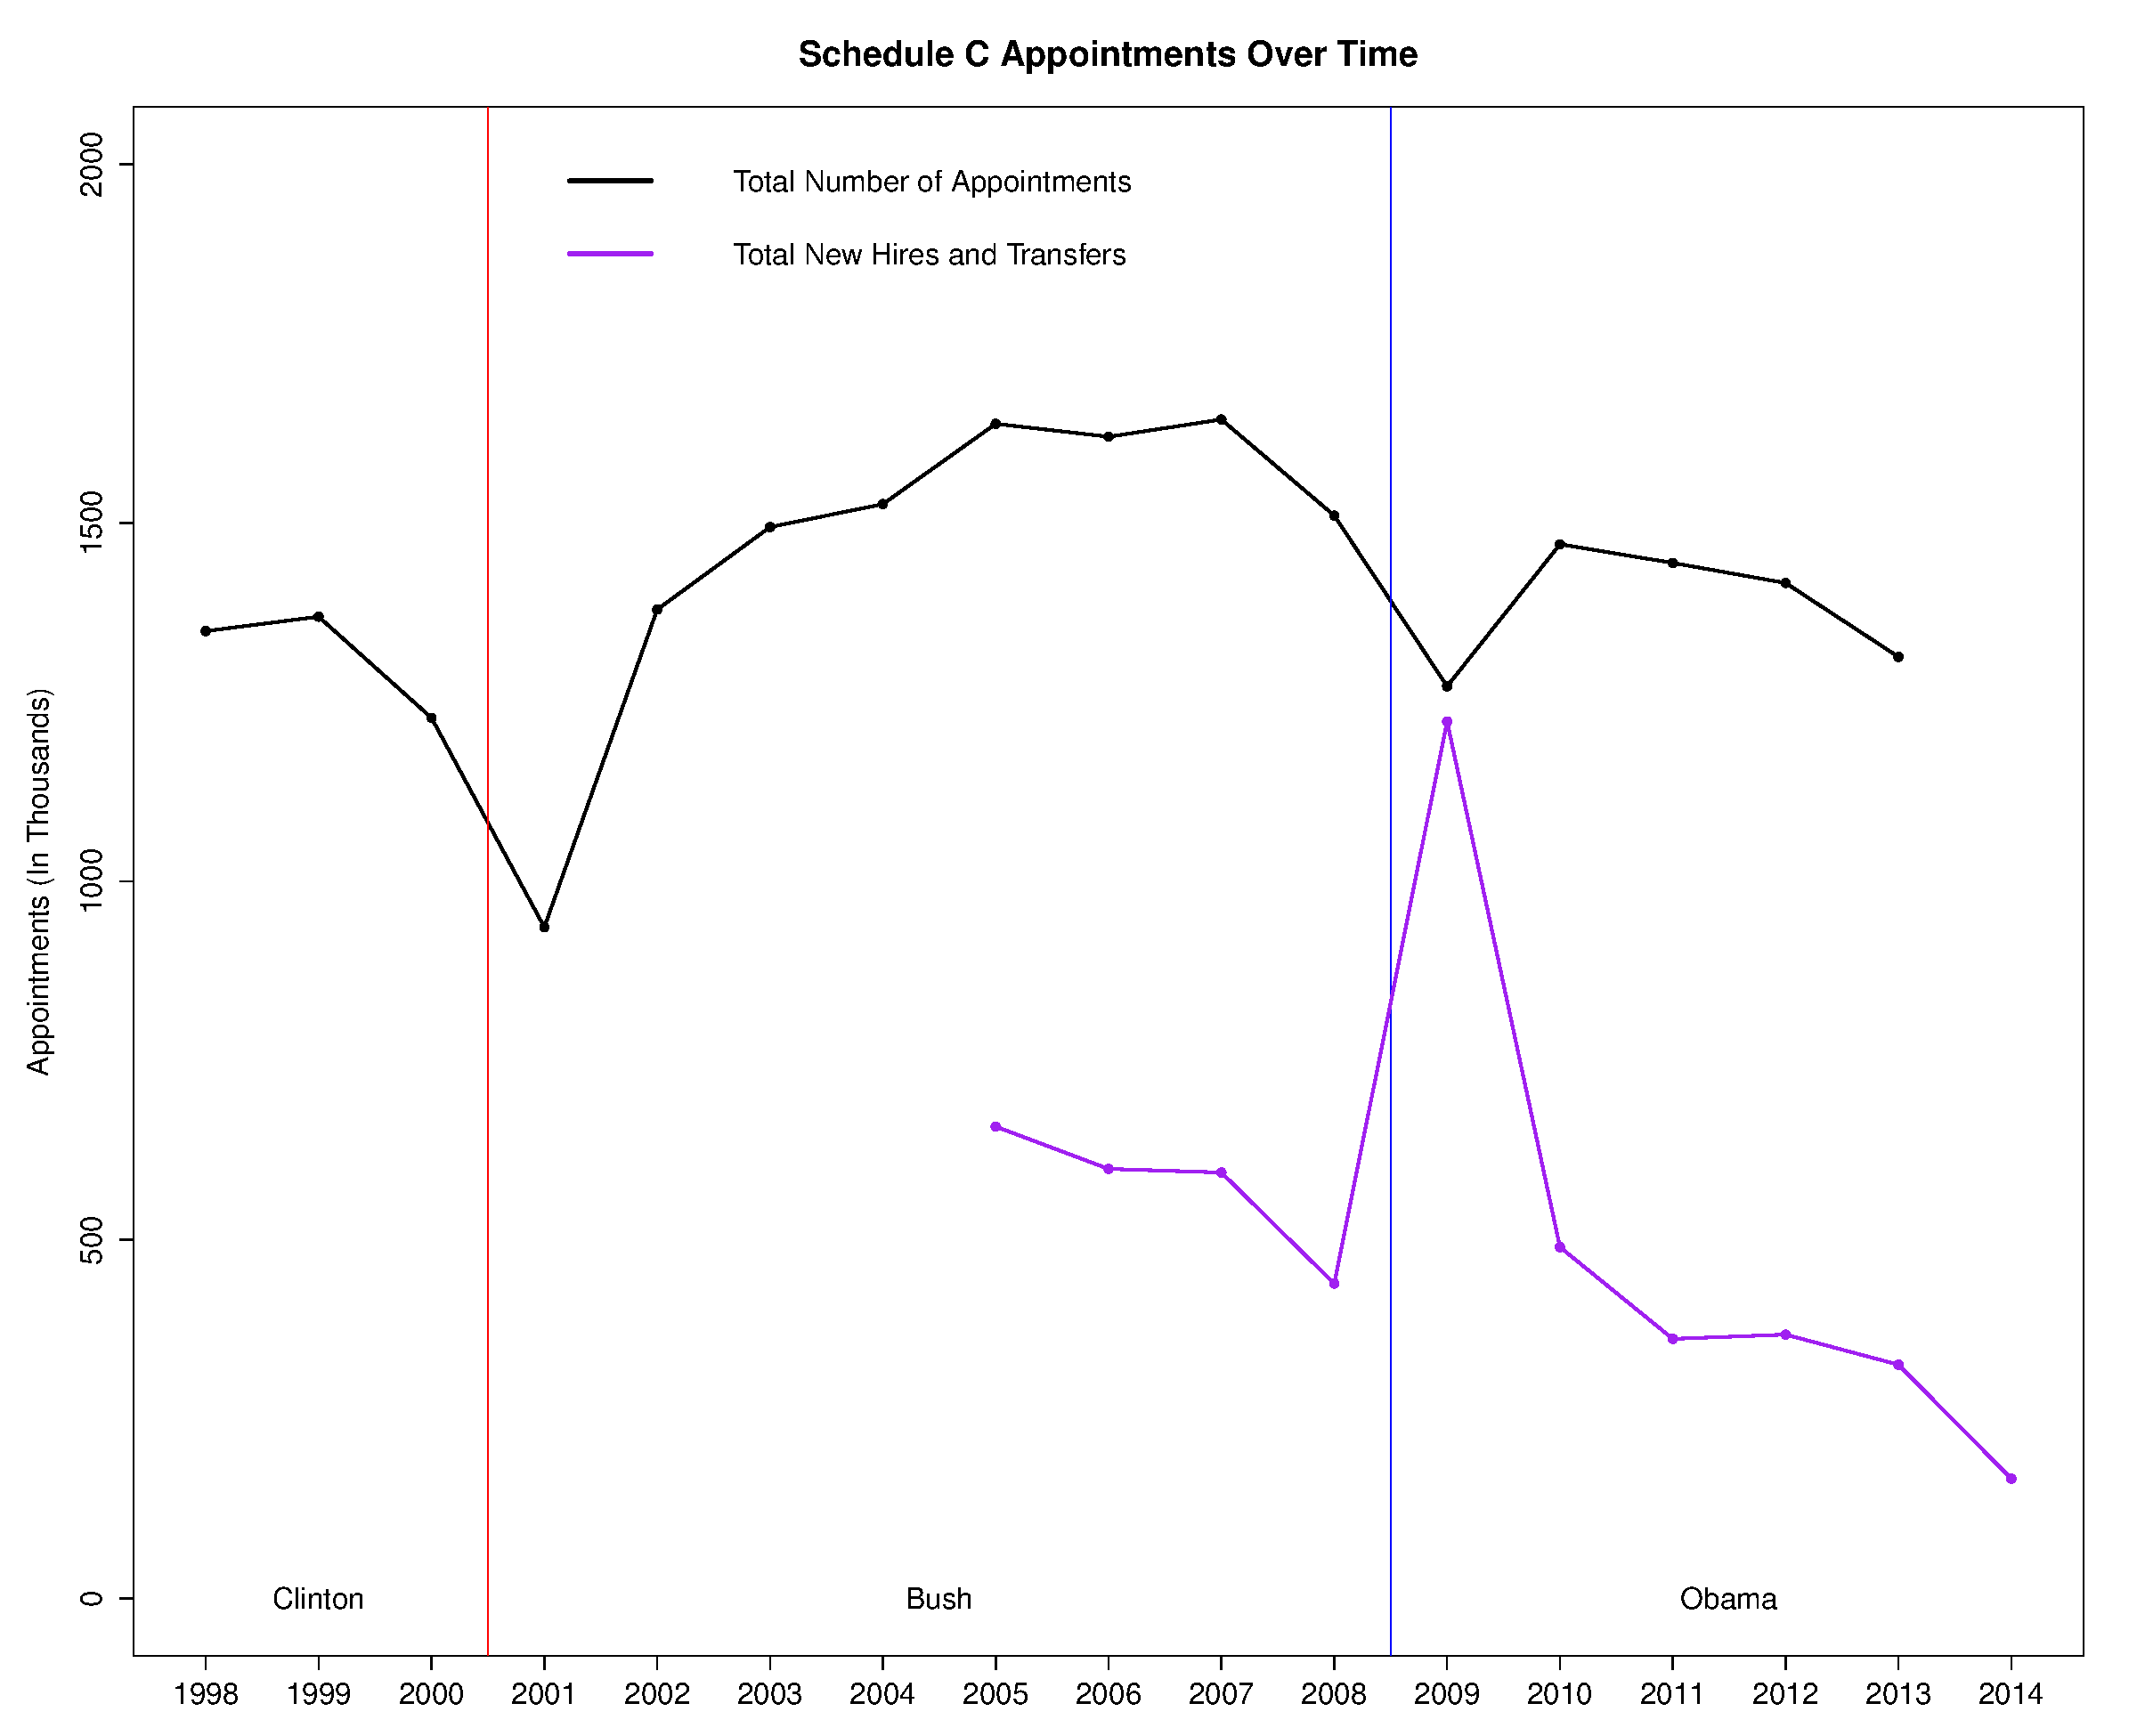
\includegraphics[height=5in,width=7in]{SCAptsandAccOverTime.pdf}
\caption{Schedule C Appointments Over Time}
\end{center}
\end{figure}

Overall, President Bush used Schedule Cs more frequently than either Clinton or Obama. In general, the number of Schedule Cs decrease and then increase when a new president takes over. As is visible, the number of accessions in 2009, when Obama takes office, is extraordinarily high---almost matching the total number of appointees in that year. While there is always some turnover during a presidential transition, this turnover is higher for political positions. The number of Schedule C accessions as a percentage of Schedule C employees is typically between 20 and 35 percent. For the Obama transition, the number of accessions as percentage of employees was over 96 percent.

%%Don't forget about extended footnote on patronage concerns. 


\section*{Flexibility and the Homeland Security Headquarters}
The Department of Homeland Security was created in direct response to 9/11. While there had been calls for the creation of a Homeland Security office earlier in 2001, it was the September 11 attacks which expedited the process. Fewer than two weeks passed before President Bush selected Governor Tom Ridge to head a new Homeland Security Office. In November of 2002, DHS was officially born as a cabinet agency by act of Congress. It began operating in March 2003 (Department Homeland Security 2014). Between the creation of a brand new cabinet department and the expediency with which President Bush pushed his agenda following the September 11 attacks and into the War on Terror, it is no surprise he would need to fill positions quickly. It is also no surprise that President Bush fought for wide discretion in DHS's creation. In fact, he used the need for expediency and discretion as a justification for his attempt to create a separate personnel system for Homeland Security that would not operate with typical civil service protections. According to the \textit{Washington Post}, Bush officials argued that the September 11 attacks required changes that would ``give more discretion to managers and permit quicker deployment of workers without notifying their union representatives" (Barr 2008). Due to their flexible nature, President Bush utilized Schedule C appointees to get the Homeland Security Headquarters up and running quickly.

Twelve Schedule C appointees were placed in the Department of Homeland Security in January of 2003. Some of these appointees were travel aids, receptionists, and scheduling assistants appointed to aid the Secretary and Undersecretary of Homeland Security in their everyday needs. Bush also appointed several speechwriters and an assistant press secretary to assist with communicating the department's messages to other agencies, Congress, and the public. Some of these early Schedule C appointees also served as special assistants who serve as advisors to the secretary and liaisons with career staff on individual policy matters. Thus, the quickly appointed Schedule Cs filled both practical and policy needs within the agency. 

Figure 3 corroborates the flexibility story. In 2003, over 40 percent of the Homeland Security Headquarters was staffed by Schedule C appointments.\footnote{The above descriptive statistics are reported with regard to the Department of Homeland Security as a whole. This figure is in reference to the Department of Homeland Security's headquarters as opposed to the entire set of subagencies within DHS.} This proportion has gradually declined ever since. In the right half of the figure we see the raw number of Schedule C appointees. The number nearly doubled from 2003 to 2004 yet the proportion of the agency employment made up by Schedule C appointees declined. This is likely because the president used Schedule C appointments to fill the department quickly, but as time went on, new hires of other appointment types came in.

\begin{figure}[!h]
\begin{center}
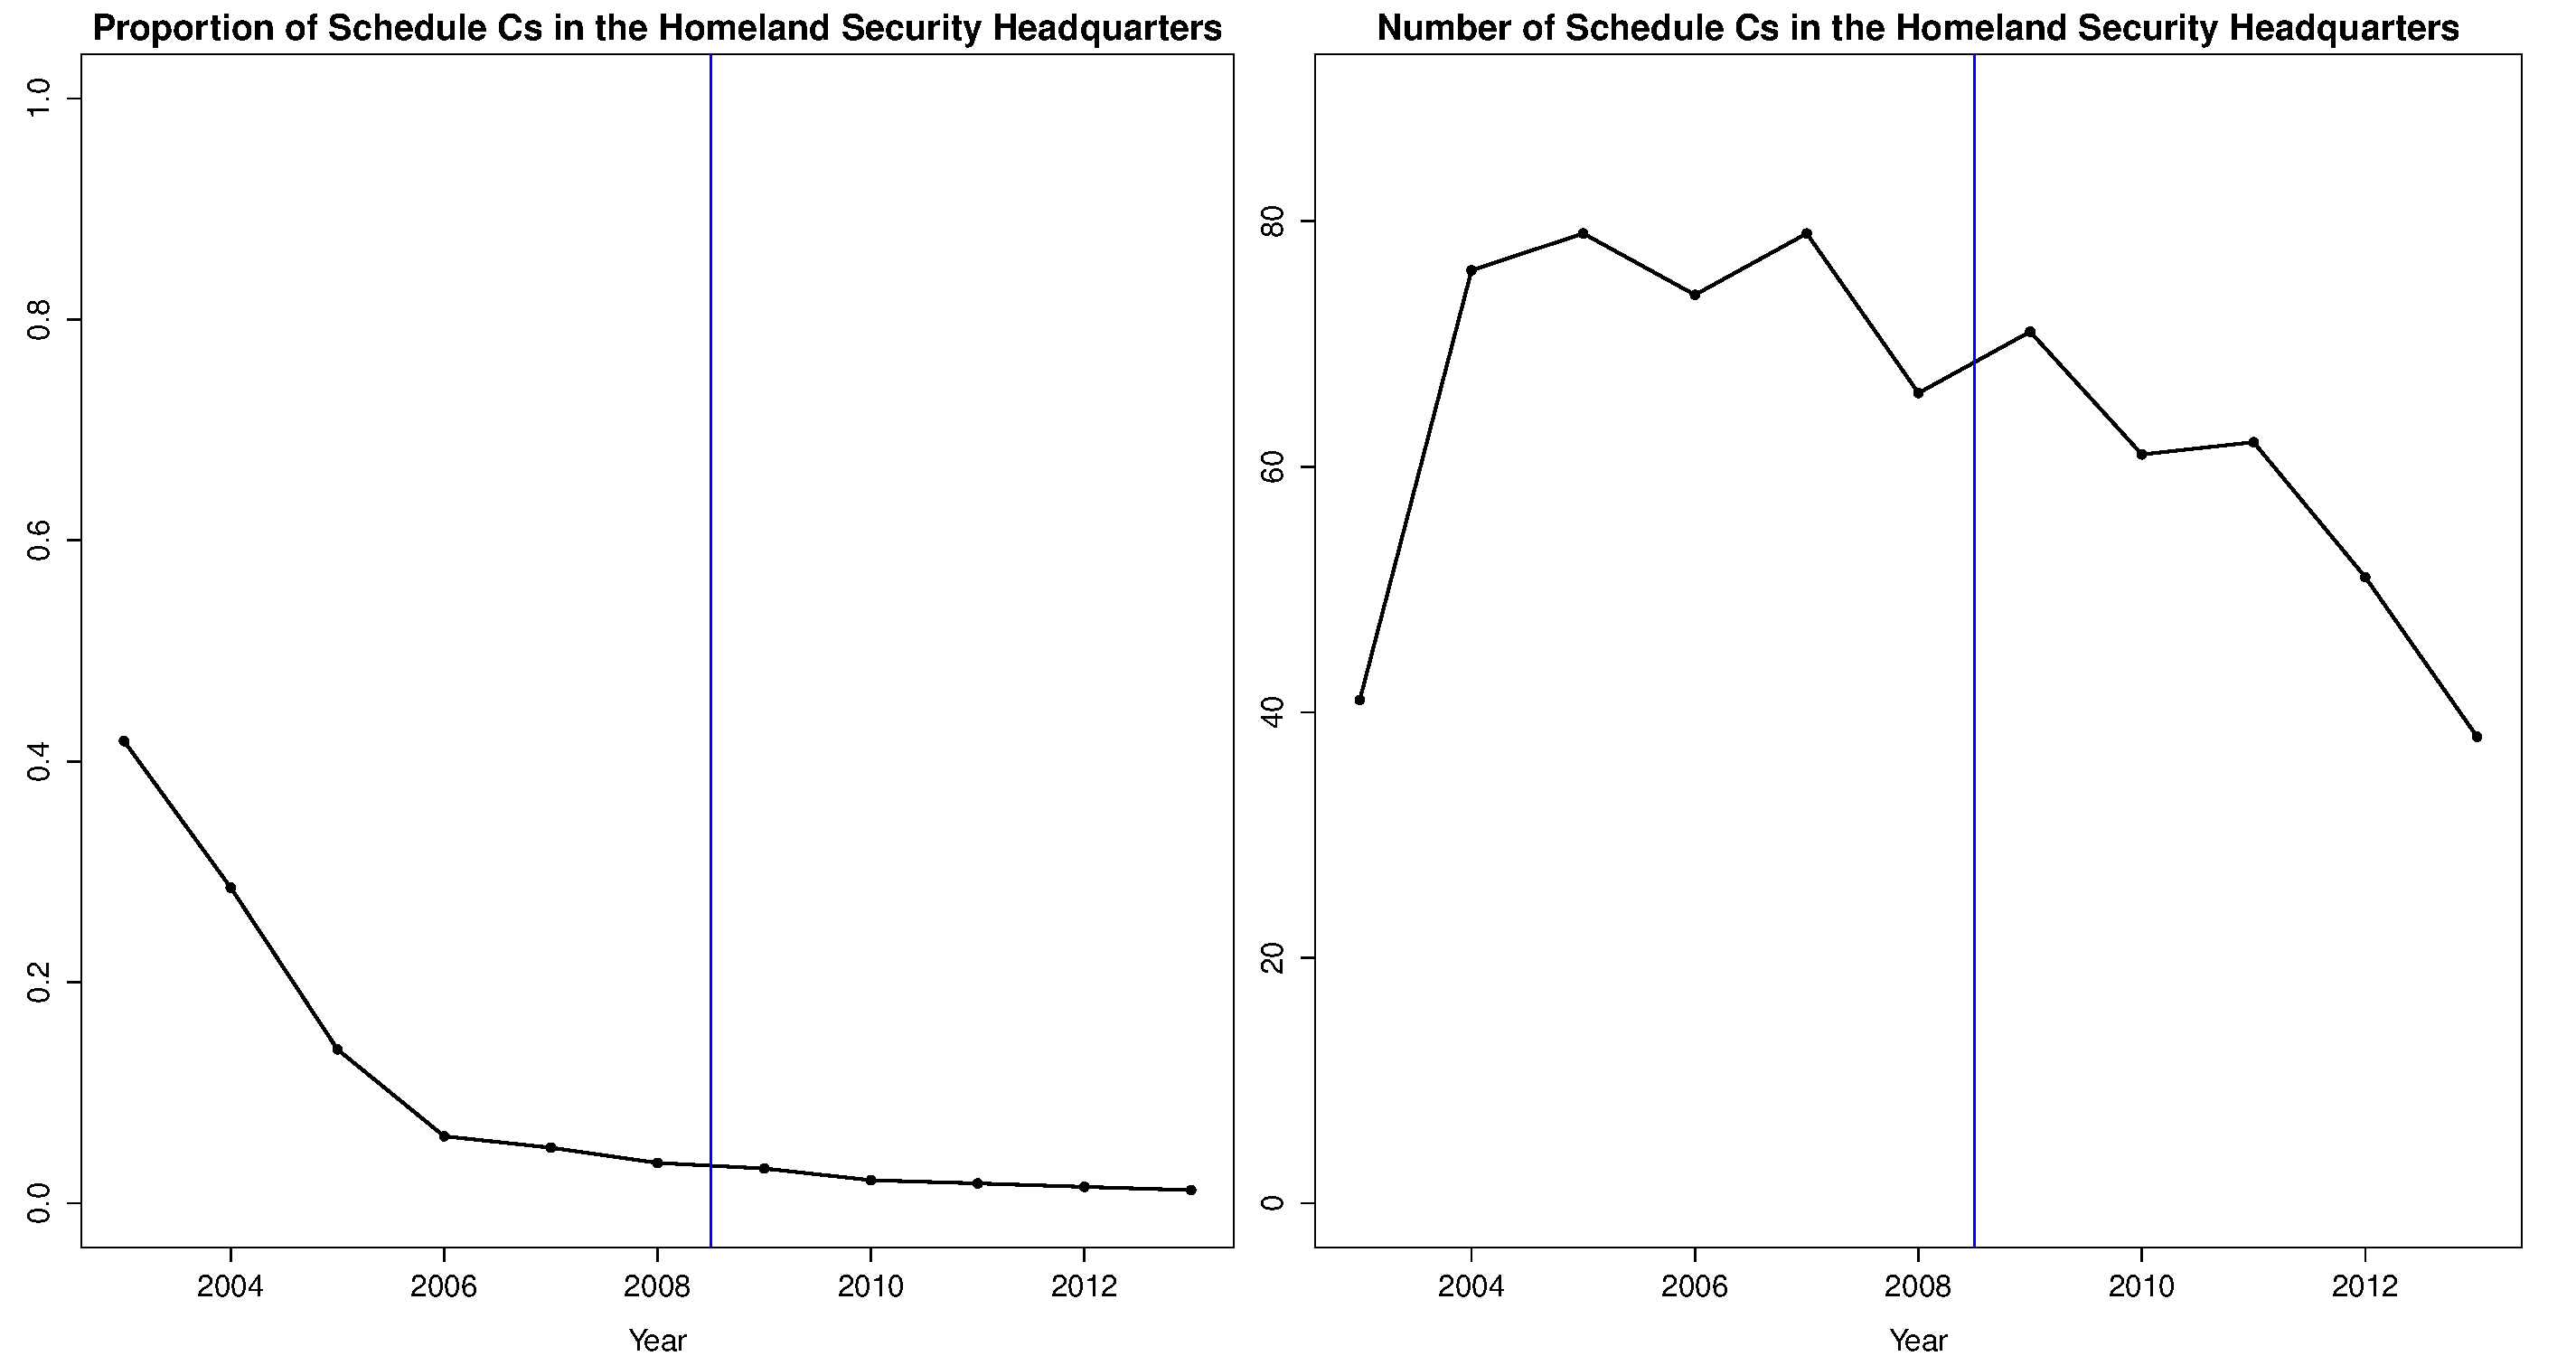
\includegraphics[height=3in,width=6in]{DHSProportionRawNumber.pdf}
\caption{Proportion and Raw Number of Schedule C and Excepted Service Executive Appointments in the Homeland Security Headquarters.}
\end{center}
\end{figure}

Importantly, these results show that presidents can and do utilize Schedule C appointees for the flexibility they provide. Rather than wait for dozens of appointees to travail through the confirmation process, the Department of Homeland Security could work for President Bush immediately. High-level officials could receive the support they needed to implement the president's agenda throughout all levels of the department rather than relying on those who may not be invested in the president's mission for the department. Most importantly, the president was able to fill these positions with the people of his choosing and do so without the fanfare that typically accompanies high-profile nominations. 


\section*{Agency Ideology and Schedule C Staffing}
To test the ideology hypothesis, I ran a negative binomial regression model predicting counts of Schedule C appointments using ideological distance of the agency from the president, controlling for the distance between party medians in the Senate and agency size, and including presidential dummies.\footnote{Distance Between Party Medians is simply the absolute DW-NOMINATE distance between the median Republican and Democrat in a given year. Agency Size is measured as the total number of appointees to an agency of all appointment types in a given year.} The outcome variable was simply the number of Schedule C appointments in an agency in a given year.

Agency ideology is measured using Chen/Johnson scores (Chen and Johnson 2015). Chen and Johnson provide agency ideology scores for each term from Clinton through Obama's first term based on federal employee campaign contributions. Importantly, these scores are scaled in common space, allowing for a comparison between the ideology of agencies and the president. Thus, the ideology measure is simply the absolute distance between an agency and the president for a given year. Chen and Johnson report 79 agencies scores. Due to differences in data coverage, this model covers 64 agencies and departments. \footnote{Most of this discrepancy comes from the fact that departments are rolled into one. Whereas Fedscope includes all the subunits of a department, those who estimate agency ideology typically estimate it for the departments as a whole. For this reason, I collapsed the appointment data for all departmental subunits into a single number for the whole department.}

The results of the two models (one with and one without clustered standard errors) are reported in Table 1. As can be seen, the coefficient for ideological distance is negative and reliable. This means that the president uses a greater number of Schedule C appointments in agencies which are ideologically similar. On average, Obama and Clinton used fewer Schedule Cs than did President Bush while larger agencies receive greater number of Schedule Cs on average. Importantly, Schedule C appointees are utilized much more frequently when the distance between party medians in the Senate is high. 

% Table created by stargazer v.5.2 by Marek Hlavac, Harvard University. E-mail: hlavac at fas.harvard.edu
% Date and time: Fri, Dec 11, 2015 - 11:56:19
\begin{table}[!htbp] \centering 
  \caption{} 
  \label{} 
\begin{tabular}{@{\extracolsep{5pt}}lcc} 
\\[-1.8ex]\hline 
\hline \\[-1.8ex] 
 & \multicolumn{2}{c}{\textit{Dependent variable:}} \\ 
\cline{2-3} 
\\[-1.8ex] & Count of Schedule Cs &   \\ 
\\[-1.8ex] & \textit{Model 1} & \textit{Model 2} \\ 
\hline \\[-1.8ex] 
 Ideological Distance & $-$2.511$^{***}$ & $-$2.511$^{***}$ \\ 
  & (0.286) & (0.446) \\ 
  & & \\ 
 Obama & $-$1.650$^{***}$ & $-$1.650$^{***}$ \\ 
  & (0.272) & (0.285) \\ 
  & & \\ 
 Clinton & $-$0.533$^{***}$ & $-$0.533$^{***}$ \\ 
  & (0.187) & (0.194) \\ 
  & & \\ 
 Distance Between Party Medians & 3.948$^{**}$ & 3.948$^{***}$ \\ 
  & (1.558) & (0.757) \\ 
  & & \\ 
 Agency Size In Thousands & 0.009$^{***}$ & 0.009$^{***}$ \\ 
  & (0.001) & (0.002) \\ 
  & & \\ 
 Constant & 1.306 & 1.306$^{***}$ \\ 
  & (1.213) & (0.417) \\ 
  & & \\ 
\hline \\[-1.8ex] 
  Clustered SEs & no & yes\\ 
\hline \\[-1.8ex] 
Observations & 811 &  \\ 
Log Likelihood & $-$3,210.314 &  \\ 
$\theta$ & 0.450$^{***}$  (0.022) &  \\ 
Akaike Inf. Crit. & 6,432.629 &  \\ 
\hline 
\hline \\[-1.8ex] 
\textit{Note:}  & \multicolumn{2}{r}{$^{*}$p$<$0.1; $^{**}$p$<$0.05; $^{***}$p$<$0.01} \\ 
\end{tabular} 
\end{table} 

Importantly, this result indicates that presidents do consider the ideology of agencies when making hiring decisions for the most flexible appointment type. Ideologically similar agencies can expect to receive much larger numbers of Schedule C appointees, suggesting that presidents utilize these appointees to bolster agencies covering policies important to them and their party. Importantly, results indicated that presidents utilize Schedule C appointees at higher levels as the distance between party medians increase. This suggests that when Congress is plagued by greater levels of polarization (and greater gridlock), the president may still be able to pursue his agenda through other means by increasing the number of appointees in ideologically similar agencies. 

\section*{Conclusion}	
When presidents reach office, they are met with the difficulty of managing an expansive bureaucratic state. They work with Congress to fill leadership positions in hundreds of agencies, but there are thousands of political appointee positions to fill. With the increasing length of time to confirmation, presidents especially need the flexibility that excepted appointments afford them. The case of the Department of Homeland Security headquarters corroborates the flexibility story. With a new cabinet department and President Bush emphasizing a sense of urgency, it is no surprise that Schedule C appointees quickly filled DHS headquarters' ranks initially, only for the proportion to decline as more positions were filled. Though the creation of a new agency in a salient policy area is an obvious place to look for an increase in excepted appointments, other research has indicated that absences in agency leadership often lead excepted appointees to take on larger roles within an agency. 

While flexibility is useful to presidents, it also behooves them to appoint ideological allies. Presidents need to fill positions at all levels of the bureaucracy in order to fully pursue their agendas. Because the president has the freedom to select the appointees of his choosing and appoint them when and where he sees fit, Schedule C appointees are an especially important tool. As I have shown, presidents tend to utilize this appointment type more frequently in ideologically similar agencies. 

Importantly, these results indicate just how important it is for bureaucratic scholars to consider a wider range of appointment types in their theories of staffing. Given how many appointees are not subject to Senate approval and given that these appointees are often involved in important decisionmaking within agencies, it is suprising they have not been given more scholarly attention. Even more broadly, it shows that scholars have been relatively narrowminded when considering presidential unilateral authority. Presidency scholars have largely focused on more obvious or tangible methods of unilateral action, but there are many ways for the president to exert his authority. This study has offered some preliminary evidence that excepted appointments are yet another method the president can use to pursue his policy agenda without Congress or in spite of it. Indeed, preliminary results indicate that the greater the distance between the party medians in Congress, the larger the number of Schedule C appointees. These results have merely skimmed the surface of how Schedule C appointees might be studied. Little is known, for example, how appointees like these might be related to tangible bureaucratic outputs such as rulemaking activity or how they are affected by transitions in agency leadership.

As Lewis and Waterman (2013) state, it is important to ``lift the veil from the president's invisible appointments." A deeper understanding of how excepted appointments fit into the broader bureaucratic system and how they are affected by the outside winds of political forces are an important step in developing a more comprehensive understanding of federal bureaucracy. This study hopes to contribute to the lifting of the veil by better understanding how these appointees can be used as an important weapon in the president's unilateral arsenal.



\section*{References}
\noindent \hangindent=0.7cm Aberbach, Joel D.,  and Bert A. Rockman. 1976. ``Clashing Beliefs withing the Executive Branch: The Nixon Administration Bureaucracy." \textit{American Political Science Review} 70(2): 456-468. 

\noindent \hangindent=0.7cm Aberbach, Joel D., and Bert A. Rockman. 1995. ``The Political Views of U.S. Senior Federal Executives, 1970-1992. \textit{Journal of Politics} 57(3): 838-52. 

\noindent \hangindent=0.7cm Aberbach, Joel D., and Bert A. Rockman. 2000. \textit{In the Web of Politics: Three Decades of the U.S. Federal Executive.} Washington, DC: Brookings.

\noindent \hangindent=0.7cm Bertelli, Anthony, and Christian Grose. 2009. ``Secretaries or Pork? A New Theory of Distributive Politics." \textit{Journal of Politics} 71(3): 926-945. 

\noindent \hangindent=0.7cm Barr, Stephen. 2008. ``DHS Withdraws Bid to Curb Union Rights." \textit{Washington Post}. \url{http://www.washingtonpost.com/wp-dyn/content/article/2008/02/1/AR2008021902459.html}. Last accessed January 6, 2014.

\noindent \hangindent=0.7cm Burke, John P. 1992. \textit{The Institutional Presidency}. Baltimore: Johns Hopkins University Press. 

\noindent \hangindent=0.7cm Chen, Jowei and Tim Johnson. 2015. "Federal employee unionization and presidential control of the bureaucracy: Estimating and explaining ideological change in executive agencies." Journal of Theoretical Politics 27(1):151-174.

\noindent \hangindent=0.7cm Clinton, Joshua D., Anthony Bertelli, Christian Grose, David E. Lewis and David C. Nixon. 2012. ``Separated Powers in the United States." American Journal of Political Science 56(2):341-54.

\noindent \hangindent=0.7cm Clinton, Joshua D., and David E. Lewis. 2008. "Expert Opinion, Agency Characteristics, and Agency Preferences." Political Analysis 16:3-20.

\noindent \hangindent=0.7cm Cohen, David M. 1988. ``Amateur Government." \textit{Journal of Public Administration Research and Theory} 8(4):450-97. 

\noindent \hangindent=0.7cm Cohen, Jeffery E. 1995. ``Presidential Rhetoric and the Public Agenda." \textit{American Journal of Political Science} 39:87-107. 

\noindent \hangindent=0.7cm Edwards III, George C. and B. Dan Wood. 1999.``Who Influences Whom? The President, Congress, and the Media." \textit{American Political Science Review} 93(2): 327-344.

\noindent \hangindent=0.7cm Eilperin, Juliet. 2014. ``Chances for Obama nominees to be confirmed are falling, even with over two years to go." \textit{Washington Post}. \url{https://www.washingtonpost.com/politics/chances-for-obama-nominees-to-be-confirmed-are-falling-even-with-over-two-years-to-go/2014/03/26/73a87b84-b107-11e3-9627-c65021d6d572_story.html}. Last accessed December 15, 2015. 

\noindent \hangindent=0.7cm Epstein, David, and Sharyn O'Halloran. 1999. \textit{Delegating Powers}. New York: Cambridge University Press. 

\noindent \hangindent=0.7cm Fenno, Richard F. 1959. \textit{The President's Cabinet: An Analysis in the Period from Wilson to Eisenhower.} Cambridge, MA: Harvard University Press.

\noindent \hangindent=0.7cm Gailmard, Sean and John W. Patty. 2012. \textit{Learning While Governing.} Chicago: University of Chicago Press. 

\noindent \hangindent=0.7cm Gilmour, John B., and David E. Lewis. 2006. ``Political Appointees and the Competence of Federal Program Management." \textit{American Politics Research} 34(1):22-50. 

\noindent \hangindent=0.7cm Harrabin, Roger. 2006.  ``Mixed Outcomes at Climate Talks." \textit{BBC}. \url{http://news.bbc.co.uk/2/hi/science/nature/5408798.stm.} Last accessed January 6, 2014.

\noindent \hangindent=0.7cm Hart, John. 1995. \textit{The Presidential Branch}.  New York: Chatham House.

\noindent \hangindent=0.7cm Heclo. 1975. ``OMB and the presidency---The problem of `neutral competence.'" \textit{Public Interest} 38(Winter): 80-98.

\noindent \hangindent=0.7cm Heclo. 1977. \textit{A Government of Strangers: Executive Politics in Washington}. Washington, DC: Brookings Institution.

\noindent \hangindent=0.7cm Hill, Kim Quaile. 1998. ``The Policy Agendas of the President and the Mass Public: A Research Validation and Extension." \textit{American Journal of Political Science}42(4): 1328-1334.

\noindent \hangindent=0.7cm Hollibaugh, Gary E. forthcoming. "Naive Cronyism and Neutral Competence: Patronage, Performance, and Policy Agreement in Executive Appointments" \textit{Journal of Public Administration Research and Theory}. 

\noindent \hangindent=0.7cm Hollibaugh Jr., Gary E., Gabe Horton, and David E. Lewis. Forthcoming. ``Presidents and Patronage." \textit{American Journal of Political Science.}

\noindent \hangindent=0.7cm Lewis, David E. 2003. \textit{Presidents and the Politics of Agency Design: Political Insulation in the United States Government Bureaucracy, 1946-1997.} Stanford, CA: Stanford University Press.

\noindent \hangindent=0.7cm Lewis, David E. 2005. ``Staffing Alone: Unilateral Action and the Politicization of the Executive Office of the President, 1988-2004." \textit{Presidential Studies Quarterly} 35(3): 496-514.

\noindent \hangindent=0.7cm Lewis, David E. 2008.\textit{The Politics of Presidential Appointments: Political Control and Bureaucratic Performance}. Princeton, NJ: Princeton University Press. 

\noindent \hangindent=0.7cm Lewis, David, E and Richard W. Waterman. 2013. ``The Invisible Presidential Appointments: An Examination of Appointments to the Department of Labor, 2001-11.'' \textit{Presidential Studies Quarterly} 43(1): 35-57.

\noindent \hangindent=0.7cm Mackenzie, G. Calvin. 1981. \textit{The Politics of Presidential Appointments}. New York: Free Press. 

\noindent \hangindent=0.7cm  Moe, Terry M. 1985. ``The Politicized Presidency." In \textit{The New Direcion in American Politics}, edited by J. E. Chubb and P.E. Peterson. Washington, DC. Brookings Institution. 

\noindent \hangindent=0.7cm O'Connell, Anne Joseph. 2008. ``Vacant Offices: Delays in Staffing Top Agency Positions" Southern California Law Review 82: 913-999.

\noindent \hangindent=0.7cm O'Connell, Anne Joseph. 2015. ``Shortening Agency and Judicial Vacancies Through Filibuster Reform? An Examination of Confirmation Rates and Delays from 1981 to 2014." \textit{Duke Law Journal} 64:1645-1715.

\noindent \hangindent=0.7cm Parsneau, Kevin. 2013. ``Politicizing Priority Departments: Presidential Priorities and Subcabinet Experience and Loyalty." \textit{American Politics Research} 41(3):443-70.

\noindent \hangindent=0.7cm Patterson, Bradley H. 2008. \textit{To Serve the President: Continuity and Innovation in the White House Staff.} Washington, DC: Brookings Institution Press.

\noindent \hangindent=0.7cm Patterson, Bradley H. and James P. Pfiffner. 2001. ``The White House Office of Presidential Personnel." \textit{Presidential Studies Quarterly} 31(3):415-438.

\noindent \hangindent=0.7cm Pfiffner, James P. 2015. ``Presidential Appointments and Managing the Executive Branch." Political Appointee Project. \url{http://www.politicalappointeeproject.org/commentary/appointments-and-managing-executive-branch} (April 9, 2015).

\noindent \hangindent=0.7cm Revkin, Andrew. 2005a. ``Bush Aide Softened Greenhouse Gas Links to Global Warming." \textit{New York Times}. \url{http://www.nytimes.com/2005/06/08/politic/08climate.html?ei=5090 &en=22149dc70c0731d8&ex=1275883200&partner=rssuserland&emc=rss.}Last Accessed January 6, 2015.

\noindent \hangindent=0.7cm Revkin, Andrew. 2005b. ``Editor of Climate Reports Resigns." \textit{New York Times}. \url{http://www.nytimes.com/2005/06/10/politics/11cooney.long.html?ex =1276056000&en=7da9d69d3b1ecb1a&ei=5090&partner=rssuserland&emc=rss&_r=0.} Last Accessed January 6, 2015. 

\noindent \hangindent=0.7cm Tolchin, Martin, and Susan Tolchin. 2010. \textit{Pinstripe Patronage: Political Favoritism from the Clubhouse to the White House and Beyond.} Boulder, CO: Paradigm Publishers.

\noindent \hangindent=0.7cm United States Agency for International Development. 2002. \textit{Performance and Accountability Report.}Washington: United States Agency for International Development.

\noindent \hangindent=0.7cm United States House of Representatives. Committee on Oversight and Government Reform. 2012. 112th 2nd. \textit{Policy and Supporting Positions}(Plum Book). 

\noindent \hangindent=0.7cm Wayne, Stephen J., Richard L. Cole, and James F.C. Hyde, Jr. 1979. ``Advising the President on Enrolled Legislation: Patterns of Executive Influence." \textit{Political Science Quarterly} 94(2): 303-16. 

\noindent \hangindent=0.7cm Wood, B. Dan and Richard W. Waterman. 1994. \textit{Bureaucratic Dynamics: The Role of Bureaucracy in a Democracy, Transforming American Politics}. Boulder: Westview Press. 


	
%Cooney story	
%	If there is any doubt left over the importance of excepted positions, consider the 2005 Cooney scandal in the Council on Environmental Quality (CEQ). The CEQ formulates reports about the status of environmental resources, reviews the environmental activities of governmental and non-governmental organizations, and oversees the implementation of the environmental impact assessment process. While the CEQ is theoretically designed such that environmental experts assess environmental impact, in reality, the process is often political. Phillip Cooney, who served in an excepted position as CEQ Chief of Staff, had only one qualification relating to the job: he had been employed as a lobbyist for the American Petroleum Institute. In 2005, a scandal broke from a report showing that Cooney purposefully doctored expert-prepared government climate reports to downplay scientific climate change findings. One anonymous EPA employee noted that, for many, Cooney's editing had damaged morale and ``created a sense of frustration'' (Revkin 2005a). The Cooney example exemplifies both the importance of excepted appointments as a political tool to advance the president's interests and the power they are able to wield over policies. 

%Miscellaneous sentences to put in other places:

%It would be easy to conclude that PAS appointees are the only bureaucrats deserving of attention. After all, there is often considerable speculation and controversy surrounding confirmation battles, and these personnel serve in some of the most important positions as cabinet secretaries and heads of independent agencies. 


\end{document}
